% !Mode:: "TeX:DE:UTF-8:Main"
%
\DocumentMetadata{
  lang        = en,
  pdfversion  = 2.0,
  pdfstandard = A-2b,
  testphase   = 
    {phase-III,
     title,
     table
	}  
}

%JOURNAL CODE  SEE DOCUMENTATION
\documentclass[ROB,biber]{nowfnt} % creates the journal version, needs biber version
%wrapper for book and ebook are created automatically.

\usepackage[utf8]{inputenc}

\usepackage{amsmath}
\usepackage{amssymb,amsfonts,amscd,amsthm}
\usepackage[printonlyused,withpage]{acronym}
% \usepackage{enumerate}

% Location of figures
 \graphicspath{{figs/}} 

% load the notation header
%!TEX root =  book.tex
% Math definitions (for use with the notation appendix)
%\newcommand{\norm}[1]{\left\Vert#1\right\Vert}
%\newcommand{\abs}[1]{\left\vert#1\right\vert}
%\newcommand{\set}[1]{\left\{#1\right\}}
%\newcommand{\Real}{\mathbb R}
%\newcommand{\Complex}{\mathbb C}
%\newcommand{\eps}{\varepsilon}
%\newcommand{\To}{\longrightarrow}
%\newcommand{\Ker}{\textup{Ker}}
%\newcommand{\Img}{\textup{Img}}
\newcommand{\diag}{\textup{diag}}
%\newcommand{\circulant}{\textup{circ}}
\newcommand{\bcf}{\;\mbox{\boldmath ${\cal F}$\unboldmath}}
%\def\Vec#1{\!\!\hbox{$#1$\kern-0.38em\lower0.85em\hbox{$\vec{}\,$}}\,}%
\newcommand{\bbm}{\begin{bmatrix}}
\newcommand{\ebm}{\end{bmatrix}}
%%\DeclareMathAlphabet{\mbf}{OT1}{ptm}{b}{n}
\newcommand{\mbf}{\mathbf}
%
%\DeclareFontFamily{OT1}{pzc}{}
%\DeclareFontShape{OT1}{pzc}{m}{it}{<-> s * [1.10] pzcmi7t}{}
%\DeclareMathAlphabet{\mathpzc}{OT1}{pzc}{m}{it}
%
\newcommand{\mbs}[1]{{\boldsymbol{#1}}}
\def\ep{\epsilon}
\def\la{\lambda}
\def\om{\omega}
\newcommand{\qc}[1]{{#1}^+}
\newcommand{\qo}[1]{{#1}^\oplus}
\newcommand{\qi}[1]{{#1}^{\scalebox{0.5}{$-1$}}}
%\newcommand{\eff}{\boxplus}
%\newcommand{\ess}{\boxtimes}
%\newcommand{\Tss}{\boxdot}
%%\newcommand{\pfs}{\boxminus}
%%\newcommand{\psf}{\Box}
%\newcommand{\pftm}{\odot}
%\newcommand{\pftp}{\circledcirc}
%\newcommand{\qm}{+}
%\newcommand{\qp}{\oplus}
%\newcommand{\eqm}{\otimes}
%\newcommand{\eqp}{\circledast}
%
%\newcommand{\mn}[3]{{#1}^{{#2}{#3}}}
%\newcommand{\rmn}[2]{\mn{\mathbb{R}}{#1}{#2}}
%
%\newenvironment{prf}[1]
%    {\textit{Proof#1:}}
%    {~\hfill $\blacksquare$\\}
%
%% Tim's Math Defs
%%\newcommand{\bcf}{\;\mbox{\boldmath ${\cal F}$\unboldmath}}
%%\def\Vec#1{\!\!\hbox{$#1$\kern-0.38em\lower0.85em\hbox{$\vec{}\,$}}\,}%
\renewcommand{\Vec}[1]{\underrightarrow{#1}}
%%\newcommand{\bbm}{\begin{bmatrix}}
%%\newcommand{\ebm}{\end{bmatrix}}
%%\DeclareMathAlphabet{\mbf}{OT1}{ptm}{b}{n}
%%\newcommand{\mbs}[1]{{\boldsymbol{#1}}}
%%\def\ep{\epsilon}
%%\def\la{\lambda}
%%\def\om{\omega}
%%\newcommand{\qc}[1]{{#1}^+}
%%\newcommand{\qo}[1]{{#1}^\oplus}
%%\newcommand{\qi}[1]{{#1}^{\scalebox{0.5}{$-1$}}}
\newcommand{\beq}{\begin{equation}}
\newcommand{\eeq}{\end{equation}}
\newcommand{\bdis}{\begin{displaymath}}
\newcommand{\edis}{\end{displaymath}}
%\newcommand{\beps}{\mbox{\boldmath $\epsilon$\unboldmath}}
\newcommand{\bomg}{\mbox{\boldmath $\omega$\unboldmath}}
\newcommand{\bfr}{\mbf{r}}
\newcommand{\bfa}{\mbf{a}}
%\newcommand{\bfv}{\mbf{v}}
\newcommand{\bfone}{\mbf{1}}
%\newcommand{\bftwo}{\mbf{2}}
\newcommand{\bfs}{\mbf{s}}
\newcommand{\bfzero}{\mbf{0}}
\newcommand{\bfC}{\mbf{C}}
\newcommand{\bfS}{\mbf{S}}
\newcommand{\bu}{{\scalebox{0.5}{\mbox{$\bullet$}}}}
\newcommand{\ci}{{\scalebox{0.5}{\mbox{$\circ$}}}}
\newcommand{\cjda}[1]{{#1}^\bu}
\newcommand{\cjdb}[1]{{#1}^\ci}
\newcommand{\cjdaa}[1]{{#1}^{\bu\bu}}
\newcommand{\cjdbb}[1]{{#1}^{\ci\ci}}
\def \bfth{\boldsymbol{\theta}}
%\def \bfep{\boldsymbol{\epsilon}}
\newcommand{\beqn}[1]{\begin{subequations}\label{eq:#1}\begin{eqnarray}}
\newcommand{\eeqn}{\end{eqnarray}\end{subequations}}
%
%\newtheorem{lemma}{Lemma}
%\newtheorem{theorem}{Theorem}
%\newtheorem{corollary}{Corollary}
%\newtheorem{remark}{Remark}
%\newtheorem{example}{Example}
%
\newcommand{\est}[1]{\hat{#1}}
\newcommand{\pri}[1]{\check{#1}}
%
%% Lie stuff
\newcommand{\wdg}{\wedge}
\newcommand{\uwdg}{\vee}
\newcommand{\Wdg}{\curlywedge}
\newcommand{\uWdg}{\curlyvee}
%
%% TRO paper
\newcommand{\pfs}{\odot}
\newcommand{\psf}{\circledcirc}
%%\newcommand{\eff}{\wedge}
%
\newcommand{\Tbig}{\mbs{\mathcal{T}}}
\newcommand{\nTbig}{\widetilde{\mbs{\mathcal{T}}}}
\newcommand{\Tsmall}{\mbf{T}}
\newcommand{\nTsmall}{\widetilde{\mbf{T}}}
%
\newcommand{\Rbig}{\mbs{\mathcal{R}}}
%
\newcommand{\Jsmall}{\mbf{J}}
\newcommand{\Jbig}{\mbs{\mathcal{J}}}
%
\newcommand{\lop}{\langle \! \langle}
\newcommand{\rop}{\rangle \! \rangle}







% a few definitions that are *not* needed in general:
\newcommand{\ie}{\emph{i.e.}}
\newcommand{\eg}{\emph{e.g.}}
\newcommand{\etc}{\emph{etc}}
\newcommand{\now}{\textsc{now}}

%ARTICLE TITLE
\title{Smoothing Out the Edges: Continuous-Time Estimation with Gaussian Process Motion Priors on Factor Graphs}


%ARTICLE SUB-TITLE
\subtitle{}


%AUTHORS FOR COVER PAGE 
% separate authors by \and, item by \\
% Don't use verbatim or problematic symbols.
% _ in mail address should be entered as \_
% Pay attention to large mail-addresses ...

%if there are many author twocolumn mode can be activated.
%\booltrue{authortwocolumn} %SEE DOCUMENTATION
\maintitleauthorlist{
Timothy D. Barfoot \\
{\sffamily\bfseries Connor Holmes} \\
{\sffamily\bfseries Zi Cong Guo} \\
{\sffamily\bfseries Sven Lilge} \\
University of Toronto \\
\and
Frank Dellaert \\
Georgia Institute of Technology
}

%ISSUE DATA AS PROVIDED BY NOW
\issuesetup
{%
 copyrightowner={T.~D.~Barfoot, C.~Holmes, Z.~C.~Guo, S.~Lilge, and F.~Dellaert},
 volume        = xx,
 issue         = xx,
 pubyear       = 2025,
 isbn          = xxx-x-xxxxx-xxx-x,
 eisbn         = xxx-x-xxxxx-xxx-x,
 doi           = 10.1561/XXXXXXXXX,
 firstpage     = 1, %Explain
 lastpage      = 18 
 }

%BIBLIOGRAPHY FILE
\addbibresource{book.bib}
\addbibresource{pubs.bib}
\addbibresource{refs.bib}

\usepackage{mwe}

%AUTHORS FOR ABSTRACT PAGE
\author[1]{Barfoot, Timothy D.}
\author[1]{Holmes, Connor}
\author[1]{Guo, Zi Cong}
\author[1]{Lilge, Sven}
\author[2]{Dellaert, Frank}

\affil[1]{University of Toronto; tim.barfoot@utoronto.ca}
\affil[2]{Georgia Institute of Technology; frank.dellaert@cc.gatech.edu}

\articledatabox{\nowfntstandardcitation}

\acrodef{BA}{Bundle Adjustment}
\acrodef{SLAM}{Simultaneous Localization and Mapping}
\acrodef{STEAM}{simultaneous trajectory estimation and mapping}
\acrodef{SDP}{Semidefinite Program}
\acrodef{IRLS}{Iteratively Reweighted Least-Squares}
\acrodef{PSD}{positive-semidefinite}
\acrodef{GP}{Gaussian Process}
\acrodef{WNOA}{White Noise on Acceleration}
\acrodef{RTS}{Rauch-Tung-Striebel}
\acrodef{KF}{Kalman filter}
\acrodef{SDE}{stochastic differential equation}
\acrodef{GN}{Gauss-Newton}
\acrodef{MAP}{maximum a posteriori}
\acrodef{BCH}{Baker-Campbell-Hausdorff}
\acrodef{LTV}{linear time-varying}
\acrodef{LTI}{linear time-invariant}



\begin{document}

\makeabstracttitle

\begin{abstract}
Continuous-time state estimation is gaining in popularity due to its abilities to provide smooth solutions, handle asynchronous sensors, and interpolate between data points.  While there are two main paradigms, {\em parametric} (e.g., temporal basis functions, splines) and {\em nonparametric} (Gaussian processes), the latter has seen less adoption despite its technical advantages and relative ease of implementation.  In this article, we seek to rectify this situation by providing a new simplified explanation of GP continuous-time estimation rooted in the language of {\em factor graphs}, which have become the de facto estimation paradigm in much of robotics.  To simplify onboarding, we also provide three working examples implemented in the popular GTSAM estimation framework.  We hope the article improves understanding and lowers the bar to entry into this exciting topic. 

\end{abstract}


%!TEX root =  FnTarticle.tex

\chapter{Introduction}
\section{What is Continuous-Time Estimation?}
\section{Parametric vs. Nonparametric}
\section{Related Work}
 
%!TEX root =  main.tex

\chapter{Factor Graph Background}
In this chapter, we will first introduce factor graphs as a general tool for formulating estimation problems.  Following this, we will work through the specific example of classic discrete-time filtering/smoothing.  We will later show that continuous-time estimation is completely compatible with this common discrete-time setup, under specific conditions.  For a more thorough introduction to factor graphs, we refer the reader to~\cite{dellaertFactorGraphsRobot2017}.

\section{Factor Graphs}
\label{sec:fg}

Typically in state estimation, we are interested in computing a posterior density representing the likelihood of a state given some inputs and measurements of the form
\begin{equation}
p(\mbf{x} | \mbf{v}, \mbf{y}),
\end{equation}
where $\mbf{x} = (\mbf{x}_0, \ldots, \mbf{x}_K)$ is the state at times $t_0, \ldots, t_K$, $\mbf{v} = (\mbf{v}_0, \ldots, \mbf{v}_K)$ is a set of inputs/commands, and $\mbf{y} = (\mbf{y}_0, \ldots, \mbf{y}_K)$ is a set of measurements.  In most practical scenarios, we can factor this posterior density into a product of factors, each of which depends on only a subset of the variables in the problem.  For example, we might have
\begin{equation}
p(\mbf{x} | \mbf{v}, \mbf{y}) \propto \underbrace{p(\mbf{x}_0)}_{\phi(\mbf{x}_0)} \prod_{k=1}^K \underbrace{p(\mbf{x}_k | \mbf{x}_{k-1}, \mbf{v}_{k,k-1})}_{\phi(\mbf{x}_{k-1},\mbf{x}_k)} \prod_{k=0}^K \underbrace{p(\mbf{y}_k | \mbf{x}_k)}_{\varphi(\mbf{x}_k)}.
\end{equation}
where each $\phi(\cdot)$, is a {\em factor} of the posterior density.  The factors can be {\em unary} (involving one variable), {\em binary} (involving two variables), or higher-order (involving more than two variables).

The normalization constant associated with this factorization is typically expensive to compute so we often satisfy ourselves with finding the $\mbf{x}$ that maximizes the posterior density, or equivalently the $\mbf{x}$ that minimizes the negative log-likelihood cost:
\begin{equation}\label{eq:cost}
\mathcal{C}(\mbf{x}) = -\log \phi(\mbf{x}_0) - \sum_{k=1}^K \log \phi(\mbf{x}_k, \mbf{x}_{k-1}) - \sum_{k=0}^K \log \varphi(\mbf{x}_k).
\end{equation}
This is a common approach in estimation, referred to as \ac{MAP} estimation.

\begin{figure}[t]
     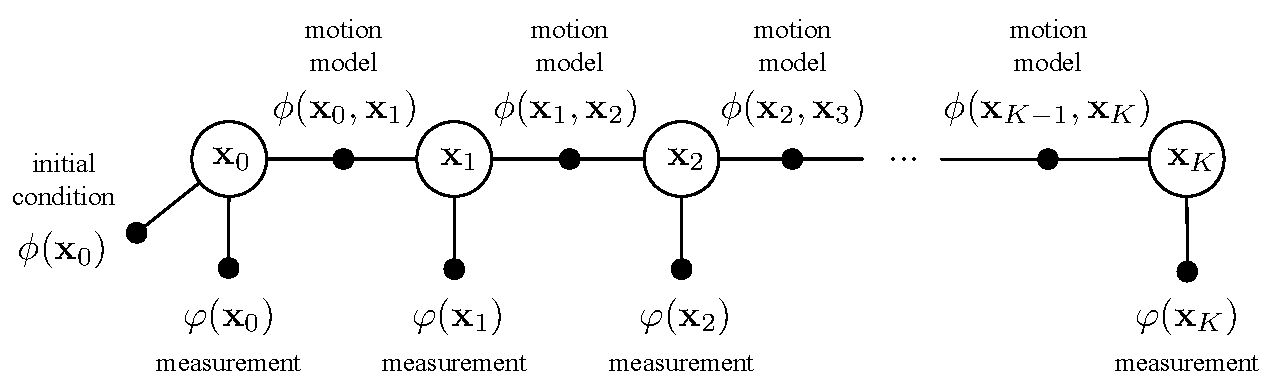
\includegraphics[width=\textwidth]{dtfg1.pdf}
     \caption{A simple factor graph for a classic estimation problem.  The unary factor on $\mbf{x}_0$ represents the prior knowledge about the initial state, the binary factors represent the motion model, and the unary factors represent the measurements.  In practice, we can have much more complicated factor graphs with loops.}
     \label{fig:dtfg1}
\end{figure}

We can visually understand the factors by assembling them into a {\em factor graph}, which is a bipartite graph with two types of nodes: variable nodes and factor nodes.  The variable nodes represent the variables in the problem, such as $\mbf{x}_0, \ldots, \mbf{x}_K$, and the factor nodes represent the factors, such as $\phi(\mbf{x}_0)$, $\phi(\mbf{x}_{k-1},\mbf{x}_k)$, and $\varphi(\mbf{x}_k)$.  The edges connect variable nodes to factor nodes, indicating which variables are involved in each factor.  This graphical representation allows us to see the dependencies between variables and factors in a very intuitive way.  Figure~\ref{fig:dtfg1} shows a simple factor graph for a classic discrete-time estimation problem.

\section{The Elimination Algorithm}

While it is possible to minimize the cost function in~\eqref{eq:cost} directly using matrix algebra, we here lean into the factor-graph representation and present the general {\em elimination algorithm}, an equivalent way to solve the minimization problem.  The key idea is to eliminate one variable at a time, updating the factors accordingly.  Once we have eliminated all variables, our factor graph has been transformed into another graph called a {\em Bayes net}; there is then a simple procedure to compute the desired posterior density from the Bayes net.

Mathematically, the elimination algorithm starts from a factor graph and ends with a new factorization of the posterior in the form
\begin{equation}\label{eq:elimfactors}
p(\mbf{x}) = p(\mbf{x}_0 | \mbf{s}_0) p(\mbf{x}_1 | \mbf{s}_1) \cdots p(\mbf{x}_K) = \prod_{k=0}^K p(\mbf{x}_k | \mbf{s}_k),
\end{equation}
where $\mbf{s}_k$ is the {\em separator} for $\mbf{x}_k$, defined as the set of variables on which $\mbf{x}_k$ is conditioned after it is eliminated.  Without loss of generality, here $k=0\ldots K$ is the order in which the variables have been eliminated. It is important to note that each variable's separator cannot include any variables that have already been eliminated, which means that once all the conditional densities are computed, we can work backwards from $K$ to $0$ to compute the posterior densities for each variable.  

Each step of the elimination algorithm consists of three operations:  (i) select a variable to eliminate, (ii) multiply all factors involving that variable together to form the {\em product factor}, and (iii) factor the product factor into a conditional density on the eliminated variable and a new factor on the separator variables.  The new factor is then added to the factor graph, and the eliminated variable is removed from the graph.  This process is repeated until all variables have been eliminated.  

In a bit more detail, consider the example factor graph on the left of Figure~\ref{fig:elim}.  Suppose we select $\mbf{x}_k$ as the variable to eliminate, then the product factor is given by
\begin{equation}
\psi(\mbf{x}_k, \mbf{s}_k) = \phi(\mbf{x}_k) \phi(\mbf{x}_k, \mbf{x}_i) \phi(\mbf{x}_k, \mbf{x}_j),
\end{equation}
where $\mbf{x}_i$ and $\mbf{x}_j$ are two other variables that share factors with $\mbf{x}_k$; the separator for $\mbf{x}_k$ is then $\mbf{s}_k = \{ \mbf{x}_i, \mbf{x}_j \}$.  The product factor is then factored into a conditional density on $\mbf{x}_k$ and a new factor on the separator variables:
\begin{equation}
\psi(\mbf{x}_k, \mbf{s}_k) = p(\mbf{x}_k | \mbf{s}_k) \, \phi(\mbf{s}_k).
\end{equation}
The key to this last factorization is that $\phi(\mbf{s}_k)$ has no dependence on $\mbf{x}_k$; it is in fact the factor that would result if $\mbf{x}_k$ were {\em marginalized} from factor graph. After all variables have been eliminated, we are left with a graph with only directed arrows called the Bayes net.

\begin{figure}[t]
     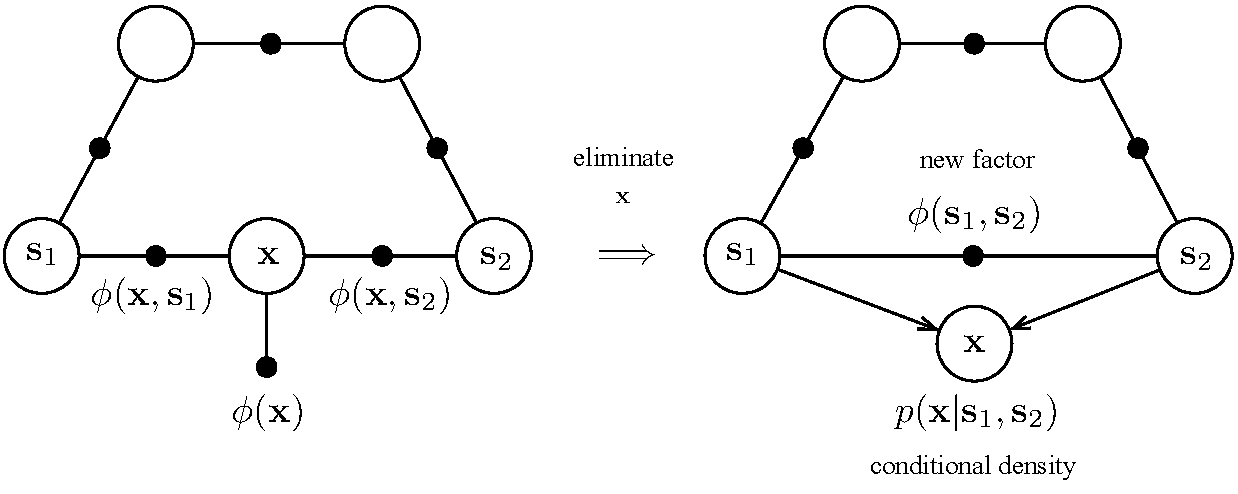
\includegraphics[width=\textwidth]{elim.pdf}
     \caption{Example of the elimination algorithm.  The left shows the factor graph before elimination, the middle shows the product factor formed by multiplying all factors involving $\mbf{x}_k$, and the right shows the result of eliminating $\mbf{x}_k$ from the factor graph, resulting in a new factor on the separator variables and a conditional density for $\mbf{x}_k$.}
     \label{fig:elim}
\end{figure}

The elimination algorithm is quite powerful in that it can be applied to any factor graph.  However, it is particularly useful for problems with a lot of structure, such as those arising in robotics, as we can exploit the sparsity of the factor graph in the various operations.  Here, we will only need to work with factors and densities that are Gaussian, and we use the next section to show that the elimination algorithm can be carried out in closed form when the factors are Gaussian.  This will allow us to carry out estimation efficiently and effectively.

\section{Gaussian Factors, Elimination, Fusion}
\label{sec:fgelimfus}

Now that we understand factor graphs and the general strategy for carrying out estimation, we show that when our factors are Gaussian we can carry out elimination in closed form.  We know that a Gaussian density has the form
\begin{equation}
p(\mbf{x}) \propto \exp\left( -\frac{1}{2} (\mbf{x} - \mbs{\mu})^T \mbs{\Sigma}^{-1} (\mbf{x} - \mbs{\mu}) \right) = \exp\left( -\frac{1}{2} || \mbf{x} - \mbs{\mu} ||^2_\mbs{\Sigma} \right).
\end{equation}
After taking the negative logarithm, we will only need the $|| \mbf{x} - \mbs{\mu} ||^2_\mbs{\Sigma}$ part, which forms a term in the negative-log likelihood cost that we are seeking to minimize; we will often then label our factors on our factor graphs using this cost term for simplicity.  We may also sometimes write $p(\mbf{x}) \sim \mathcal{N}(\mbs{\mu}, \mbs{\Sigma})$ as a shorthand for Gaussian densities.

\begin{figure}[t]
     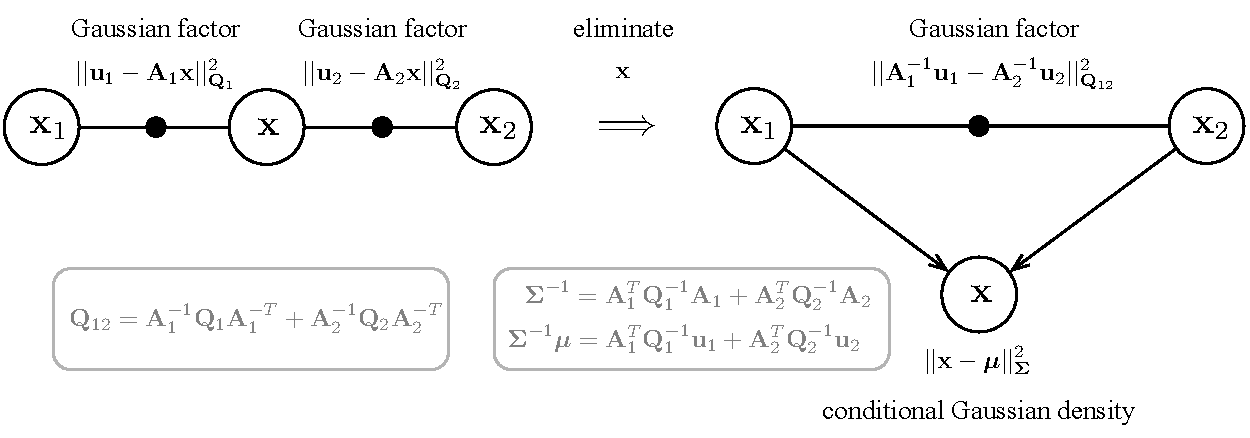
\includegraphics[width=\textwidth]{gausselim.pdf}
     \caption{With Gaussian factors, eliminating $\mbf{x}$ results in a new Gaussian factor and a Gaussian conditional density for $\mbf{x}$.}
     \label{fig:gausselim}
\end{figure}

Consider the situation on the left of Figure~\ref{fig:gausselim}; we have $\mbf{x}$ linked to two other variables via Gaussian factors (i.e., $\mbf{x}$'s separator).  When we eliminate $\mbf{x}$, this results in the situation on the right, with a new binary factor between the separator variables as well as a Gaussian conditional density for $\mbf{x}$.  Note, we assume that $\mbf{u}_1$ depends on $\mbf{x}_1$ and $\mbf{u}_2$ depends on $\mbf{x}_2$, typically linearly, but the elimination procedure still works if $\mbf{x}$ has a binary factor on one side and a unary factor on the other. 

The Gaussian elimination in Figure~\ref{fig:gausselim} follows from the very handy sum-of-squares identity,
\begin{equation}\label{eq:sumofsquares}
|| \mbf{u}_1 - \mbf{A}_1 \mbf{x} ||^2_{\mbf{Q}_1} + || \mbf{u}_2 - \mbf{A}_2 \mbf{x} ||^2_{\mbf{Q}_2}  = || \mbf{A}_1^{-1} \mbf{u}_1 - \mbf{A}_2^{-1} \mbf{u}_2 ||^2_{\mbf{Q}_{12}} + || \mbf{x} - \mbs{\mu}||^2_\mbs{\Sigma},
\end{equation}
where $\mbf{Q}_{12}$, $\mbs{\Sigma}$, $\mbs{\mu}$,  are defined in Figure~\ref{fig:gausselim} and $\mbf{A}_1$ and $\mbf{A}_2$ are for now assumed invertible.  We will use this closed-form Gaussian elimination time and again in what follows.  

\begin{figure}[t]
     \centering
     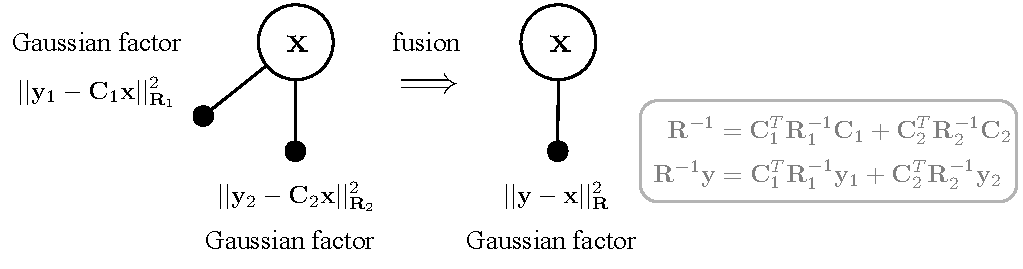
\includegraphics[width=0.8\textwidth]{gaussfusion.pdf}
     \caption{We can fuse multiple Gaussian factors into a single one in order to declutter our factor graph.}
     \label{fig:gaussfusion}
\end{figure}

Another operation that we will perform frequently with Gaussian factors is fusion.  By this we mean lumping together multiple factors into a single one as depicted in Figure~\ref{fig:gaussfusion} for unary factors.  In fact, it is a well-known result that we can fuse an arbitrary number of Gaussians in this way, allowing us to declutter our factor graph.

We are now prepared to discuss classic discrete-time estimation from a factor-graph perspective.

\section{Linear Discrete-Time Estimation}
\label{sec:ldte}

Classic discrete-time state estimation has a chain-like factor graph as depicted in Figure~\ref{fig:dtfg1}.  There is a unary initial-condition factor capturing what we know about the state at the initial time, binary motion-model factors predicting how the system moves from one discrete time to the next, and unary measurement factors that tell us something about the state at each discrete time. 

% \begin{figure}[b]
%      \centering
%      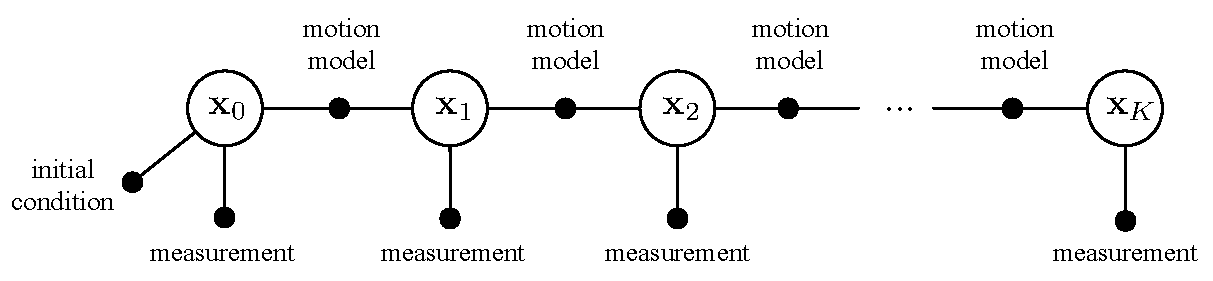
\includegraphics[width=0.95\textwidth]{dtfg.pdf}
%      \caption{Factor graph for classic discrete-time filtering/smoothing estimators.}
%      \label{fig:dtfg}
% \end{figure}

For example, we might have a stochastic linear system of the form
\beqn{linsys}
\mbf{x}_k & = & \mbf{A}_{k,k-1} \mbf{x}_{k-1} + \mbf{v}_{k,k-1} + \mbf{w}_{k,k-1},  \\
\mbf{y}_k & = & \mbf{C}_k \mbf{x}_k + \mbf{n}_k,
\eeqn
where $k \in 0 \ldots K$ is the discrete-time index, $\mbf{x}_k$ is the state, $\mbf{v}_{k,k-1}$ is an input/command, $\mbf{y}_k$ is an output/measurement, $\mbf{w}_{k,k-1} \sim \mathcal{N}(\mbf{0}, \mbf{Q}_{k,k-1})$ is Gaussian process noise, and $\mbf{n}_k \sim \mathcal{N}(\mbf{0}, \mbf{R}_k)$ is Gaussian measurement noise.  We additionally assume that at $k=0$ the initial condition is drawn from a Gaussian, $\mbf{x}_0 \sim \mathcal{N}\left(\pri{\mbf{x}}_0, \pri{\mbf{P}}_0\right)$.  In this case, we can populate our factor graph as in Figure~\ref{fig:dtfg2}, where all of the factors are now Gaussian.  

An important point to make when looking at Figure~\ref{fig:dtfg2} is that the factor graph has a lot of structure in the form of sparsity.  Not all nodes are connected to all other nodes; rather, each node is connected only to its temporal neighbours.  This sparsity arises because $\mbf{x}$ is a {\em Markovian} state for~\eqref{eq:linsys}.  In other words, it captures everything we need to know to predict the next state of the system.  

Our state-estimation problem is now to use the initial-state knowledge, $\pri{\mbf{x}}_0$, the inputs, $\mbf{v}_{k,k-1}$, and the measurements, $\mbf{y}_k$, to work out the likelihood of $\mbf{x}$ taking on all possible values.   This can be done exactly for this linear-Gaussian system; later for nonlinear systems we will require some approximations.  We will show that by using a combination of the Gaussian elimination and fusion operations from Section~\ref{sec:fgelimfus}, we can recover the classic \ac{RTS} smoother, the forward pass of which is the famous \ac{KF}.

\begin{figure}[t]
     \centering
     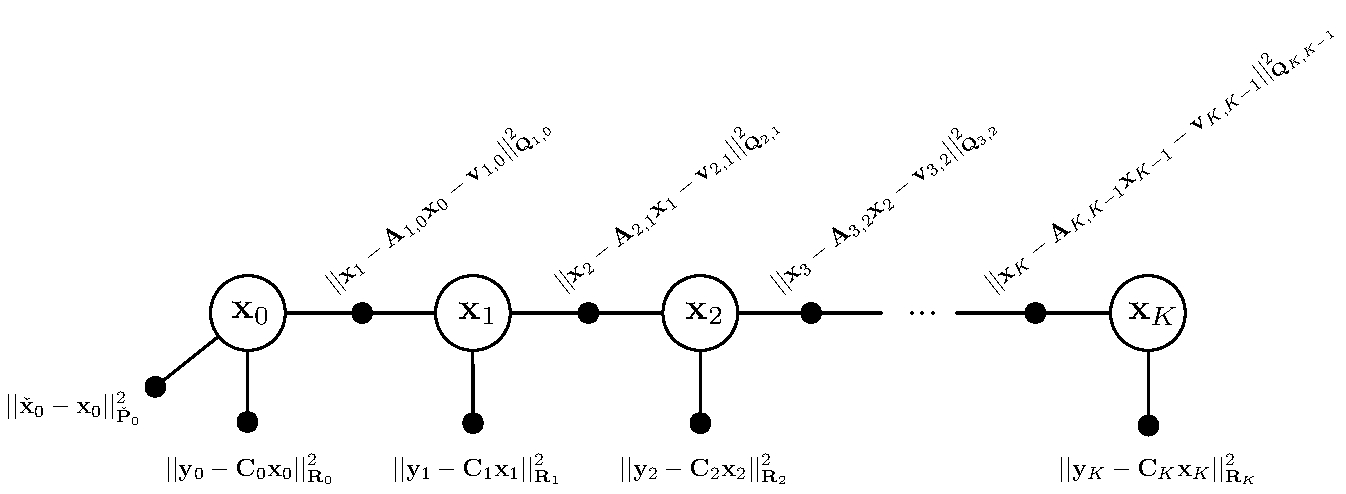
\includegraphics[width=\textwidth]{dtfg2.pdf}
     \caption{Populated factor graph for the discrete-time estimation of the linear system in~\eqref{eq:linsys}.}
     \label{fig:dtfg2}
\end{figure}

Looking to Figure~\ref{fig:dtfg2}, our estimation game plan will be to first fuse the two unary factors on $\mbf{x}_0$, then eliminate $\mbf{x}_0$, then repeat this process with $\mbf{x}_1$ and so on until we arrive at $\mbf{x}_K$.  The result of this forward pass will be a Bayes net.  After this we will carry out a backward pass to work out the posterior densities for $\mbf{x}_K$ all the way back to $\mbf{x}_0$.

\begin{figure}[p]
     \centering
     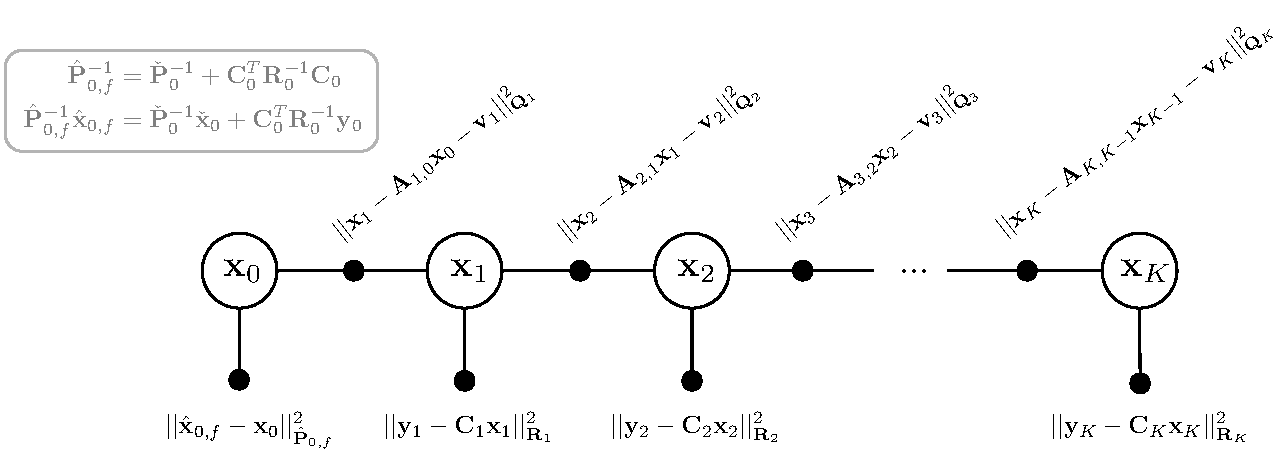
\includegraphics[width=\textwidth]{dtfg3.pdf}
     \caption{Result after fusing the two unary factors on $\mbf{x}_0$ in Figure~\ref{fig:dtfg2}.}
     \label{fig:dtfg3}
\end{figure}
\begin{figure}[p]
     \centering
     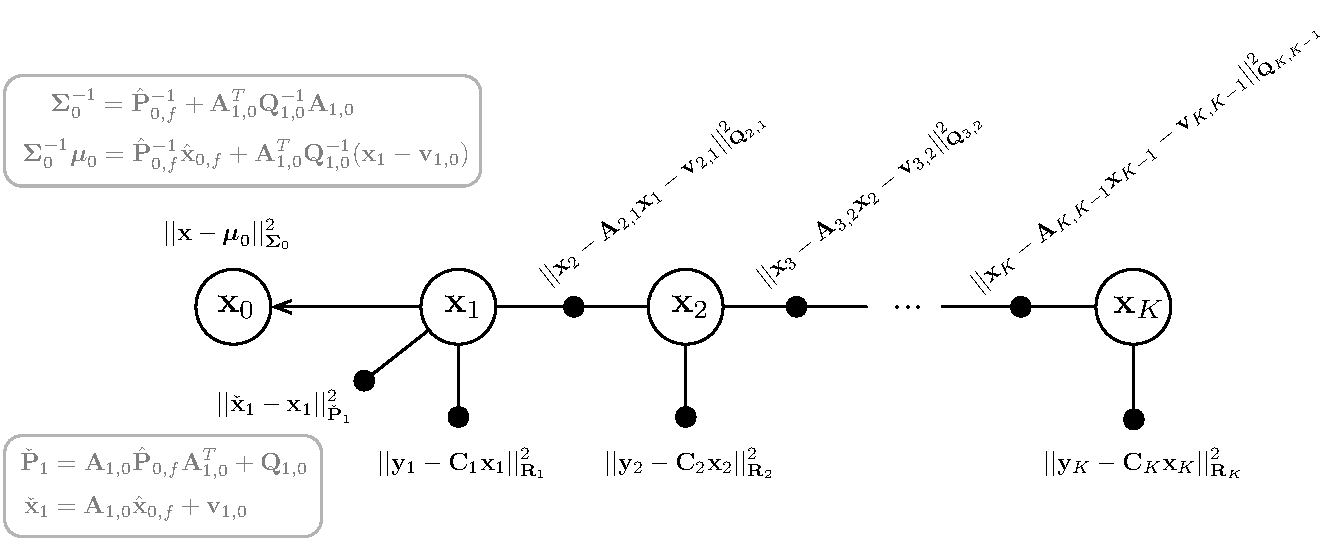
\includegraphics[width=\textwidth]{dtfg4.pdf}
     \caption{Result after eliminating $\mbf{x}_0$ from the factor graph in Figure~\ref{fig:dtfg3}.}
     \label{fig:dtfg4}
\end{figure}
\begin{figure}[p]
     \centering
     \hspace*{0.5in}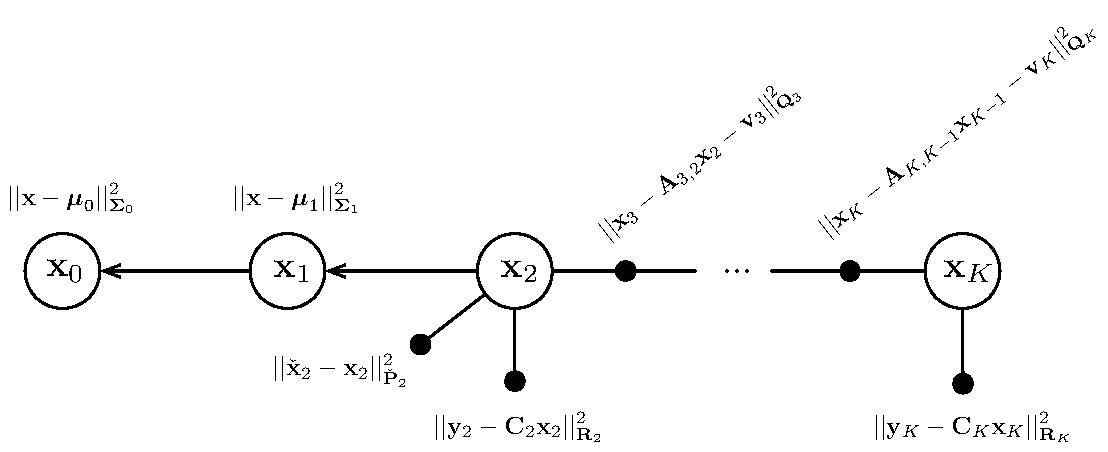
\includegraphics[width=0.87\textwidth]{dtfg5.pdf}
     \caption{Result after fusing the two unary factors on $\mbf{x}_1$ in Figure~\ref{fig:dtfg4} and then also eliminating $\mbf{x}_1$.}
     \label{fig:dtfg5}
\end{figure}

Figure~\ref{fig:dtfg3} shows the result of fusing the two unary factors on $\mbf{x}_0$ into a single Gaussian factor.  Figure~\ref{fig:dtfg4} then shows the result of eliminating $\mbf{x}_0$ from the factor graph, resulting in a new unary factor on $\mbf{x}_1$ as well as the conditional density for $\mbf{x}_0$.  We now notice that the remaining factor graph looks identical to the one we started with, only shifted forward by one time step.  Figure~\ref{fig:dtfg5} shows what happens after another round of fusing the unary factors on $\mbf{x}_1$ then eliminating $\mbf{x}_1$.  If we keep applying this same procedure all the way to time step $K$, our factor graph is completely eliminated and we are left with the Bayes net in Figure~\ref{fig:dtfg6}.  We can then work backward from $\mbf{x}_K$ back to $\mbf{x}_0$ using the conditional densities to compute the posterior densities for each state.

\begin{figure}[t]
     \centering
     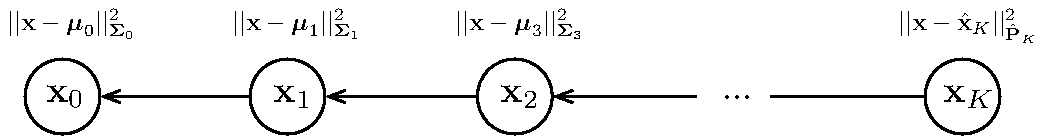
\includegraphics[width=0.85\textwidth]{dtfg6.pdf}
     \caption{After eliminating all the variables in a forward pass, we are left with a Bayes net.  We can then carry out a backward pass to calculate the posterior densities on all the variables.}
     \label{fig:dtfg6}
\end{figure}

After some algebraic manipulations, it can be shown that this procedure is identical to the classic \ac{RTS} smoother, consisting of the same forward and backward passes:
\begin{subequations}
\label{eq:rts}
\begin{eqnarray}
\mbox{forward:} \quad\;\;\; & & \nonumber \\
\mbox{($k=1\ldots K$)} \; & & \nonumber \\
\pri{\mbf{P}}_{k,f} & = & \mbf{A}_{k,k-1} \est{\mbf{P}}_{k-1,f} \mbf{A}_{k,k-1}^T + \mbf{Q}_{k,k-1}, \\
\pri{\mbf{x}}_{k,f} & = & \mbf{A}_{k,k-1} \est{\mbf{x}}_{k-1,f} + \mbf{v}_{k,k-1}, \\
\mbf{K}_k & = & \pri{\mbf{P}}_{k,f} \mbf{C}_k^T \left( \mbf{C}_k \pri{\mbf{P}}_{k,f} \mbf{C}_k^T + \mbf{R}_k \right)^{-1}, \\
\est{\mbf{P}}_{k,f} & = & \left( \mbf{1} - \mbf{K}_k \mbf{C}_k \right) \pri{\mbf{P}}_{k,f}, \\
\est{\mbf{x}}_{k,f} & = & \pri{\mbf{x}}_{k,f} + \mbf{K}_k \left( \mbf{y}_k - \mbf{C}_k \pri{\mbf{x}}_{k,f} \right), \\
\mbox{backward:}\quad & & \nonumber \\
\mbox{($k=K\ldots 1$)} \; & & \nonumber \\
\est{\mbf{x}}_{k-1} & = & \est{\mbf{x}}_{k-1,f} + \left(\est{\mbf{P}}_{k-1,f} \mbf{A}_{k,k-1}^T \pri{\mbf{P}}_{k,f}^{-1} \right)\left( \est{\mbf{x}}_k - \pri{\mbf{x}}_{k,f} \right), \qquad\quad \\
\est{\mbf{P}}_{k-1} & = & \est{\mbf{P}}_{k-1,f} + \left( \est{\mbf{P}}_{k-1,f} \mbf{A}_{k,k-1}^T \pri{\mbf{P}}_{k,f}^{-1}\right) \left( \est{\mbf{P}}_k - \pri{\mbf{P}}_{k,f} \right) \nonumber \\  &  & \qquad\qquad\qquad\quad \times \; \left( \est{\mbf{P}}_{k-1,f} \mbf{A}_{k,k-1}^T \pri{\mbf{P}}_{k,f}^{-1}\right)^T \label{eq:rtsbackcov3}, 
\end{eqnarray}
\end{subequations}
which are initialized with 
\begin{subequations}
\begin{eqnarray}
\est{\mbf{P}}_{0,f} & = & ( \mbf{1} - \mbf{K}_0 \mbf{C}_0 ) \pri{\mbf{P}}_0, \\
\est{\mbf{x}}_{0,f} & = & \pri{\mbf{x}}_0 + \mbf{K}_0 ( \mbf{y}_0 - \mbf{C}_0 \pri{\mbf{x}}_0), \\
\est{\mbf{x}}_K & = & \est{\mbf{x}}_{K,f}, \\
\est{\mbf{P}}_K & = & \est{\mbf{P}}_{K,f},
\end{eqnarray}
\end{subequations}
and $\mbf{K}_0 = \pri{\mbf{P}}_{0} \mbf{C}_0^T \left( \mbf{C}_0 \pri{\mbf{P}}_{0} \mbf{C}_0^T + \mbf{R}_0 \right)^{-1}$.  We will also be interested in computing the cross-covariance between two consecutive states, which is given by
\begin{equation}
\est{\mbf{P}}_{k,k-1} = \est{\mbf{P}}_{k} \left( \est{\mbf{P}}_{k-1,f} \mbf{A}_{k,k-1}^T \pri{\mbf{P}}_{k,f}^{-1}\right)^T
\end{equation}
and can be calculated during the backward pass.  The computational complexity of the \ac{RTS} smoother is $O(K)$, in other words, linear in the length of the trajecotry.

The forward pass is the very famous \acf{KF}, which we now understand from a factor-graph perspective.  The $p(\mbf{x}_k | \mbf{v}_{0:k}, \mbf{y}_{0:k}) = \mathcal{N}\left(\est{\mbf{x}}_{k,f}, \est{\mbf{P}}_{k,f} \right)$ quantities can be referred to as {\em filtered} (accounting only for up-to-the-present measurements) while the $p(\mbf{x}_k | \mbf{v}_{0:K}, \mbf{y}_{0:K}) = \mathcal{N}\left( \est{\mbf{x}}_k, \est{\mbf{P}}_k \right)$ quantities are {\em smoothed} (accounting for all measurements: past, present, and future); see Figure~\ref{fig:filtersmoother}.

\begin{figure}[b]
     \centering
     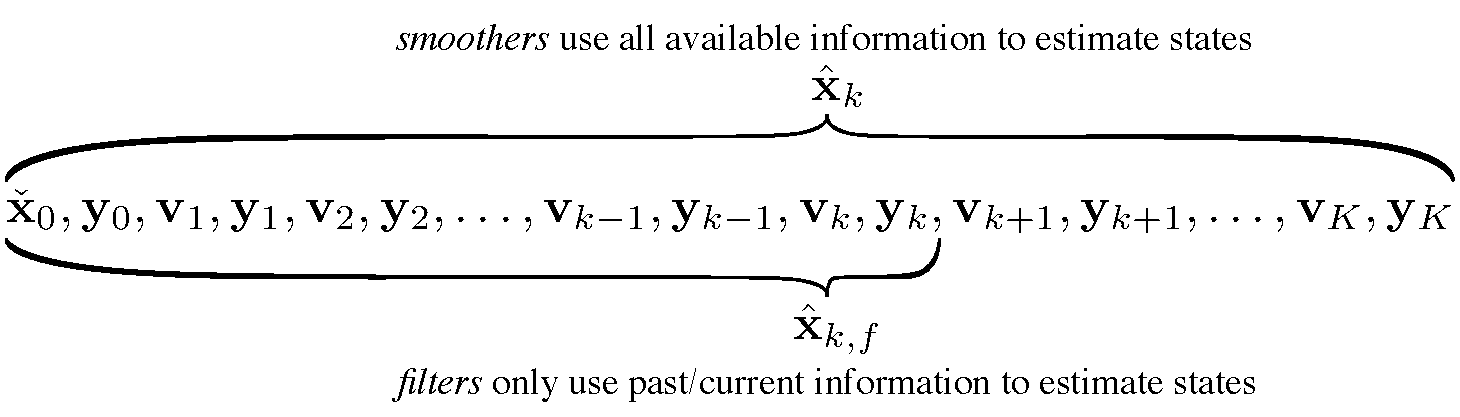
\includegraphics[width=0.95\textwidth]{filtersmoother.pdf}
     \caption{Contrasting filtering vs. smoothing.  We are primarily interested in smoothing in this article.}
     \label{fig:filtersmoother}
\end{figure}

It turns out that this discrete-time estimation setup is completely compatible with extending our results to continuous time, we just need to fill in the details of~\eqref{eq:linsys} in the right way.  This will be the subject of the next chapter.



%!TEX root =  FnTarticle.tex

\chapter{Continuous-Time Linear Systems}

In this chapter, we show how to carry out so-called {\em continuous-time} estimation.  What we really mean by this is that we have some measurements at specific times that we should use to estimate the trajectory at some query times; the query times and the estimation times need not be the same.  Figure~\ref{fig:ctfg} shows the situation in which we are interested, with a single query time.

\begin{figure}[b]
     \centering
     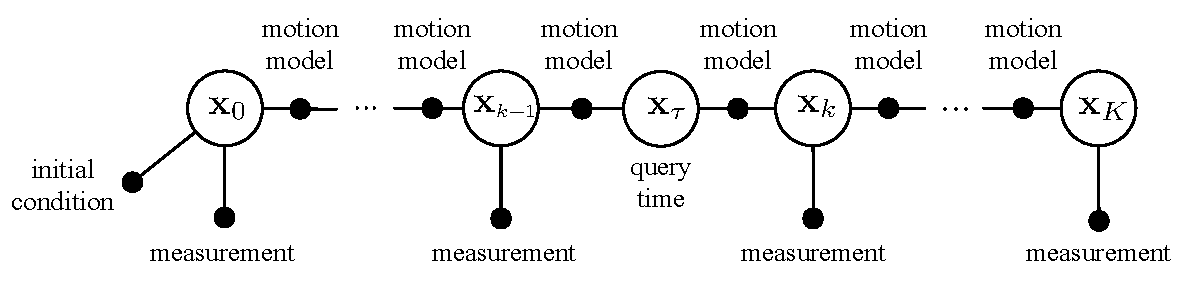
\includegraphics[width=0.95\textwidth]{ctfg.pdf}
     \caption{A continuous-time estimation problem with measurements at discrete times and a single query time.  We refer to this as `continuous-time' because the query(ies) could be at any time along the trajectory.}
     \label{fig:ctfg}
\end{figure}

We will see that we can recycle what we learned in the previous chapter for discrete-time estimation when approaching the continuous-time problem in Figure~\ref{fig:ctfg}.  In a nutshell, we can break the problem down into two main steps:
\begin{enumerate}
\item {\em main solve}: solve for the states at the measurement times
\item {\em interpolation}: solve for the states at the query times
\end{enumerate}
The key to this decomposition is to again use the elimination algorithm to remove the query state from the factor graph, resulting in the situation in Figure~\ref{fig:ctfg2}.  The remaining factor graph is now identical in structure to the one treated in the previous chapter; we can therefore solve at the measurement times and then the query time.  The next two sections work through the details.

\begin{figure}[t]
     \centering
     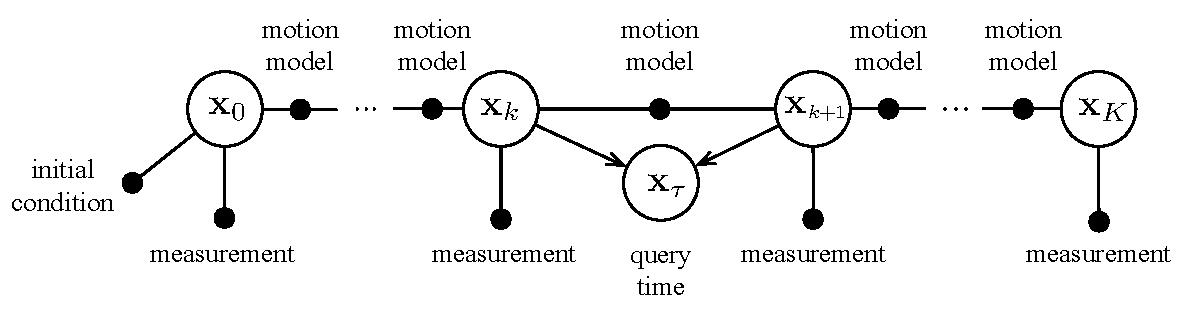
\includegraphics[width=0.95\textwidth]{ctfg2.pdf}
     \caption{The same factor graph as Figure~\ref{fig:ctfg} with the state at the query time, $\mbf{x}_\tau$, eliminated.}
     \label{fig:ctfg2}
\end{figure}

\section{Main Solve}

The first step in our strategy is to solve for the states at the measurement times in Figure~\ref{fig:ctfg2}.  This is precisely the problem discussed in the previous chapter and so we already know how to carry this out.  However, we would like our solution to obey an important property:  whether we solve the factor-graph problem in Figure~\ref{fig:ctfg} ($\mbf{x}_\tau$ estimated during the main solve) or the one in Figure~\ref{fig:ctfg2} ($\mbf{x}_\tau$ computed afterwards), the solutions should agree.  This comes down to choosing the details of the motion model appropriately.

We previously had a discrete-time motion model, but now we will start with a generic continuous-time one:
\begin{equation}\label{eq:linsysct}
\dot{\mbs{x}}(t) = \mbs{A} \mbs{x}(t) + \mbs{v}(t) + \mbs{L} \mbs{w}(t),
\end{equation}
where $\mbs{x}(t)$ is the state, $\mbs{v}(t)$ the input, and $\mbs{w}(t) \sim \mathcal{GP}(\mbf{0}, \mbs{Q} \delta(t-t^\prime))$ a white-noise process.  For example if we choose the coefficient matrices to be $\mbs{A} = \bbm \mbf{0} & \mbf{I} \\ \mbf{0} & \mbf{0} \ebm$ and $\mbs{L} = \bbm \mbf{0} \\ \mbf{I} \ebm$ and set the inputs to zero, $\mbs{v}(t) = \mbf{0}$, then our state represents position and velocity, $\mbs{x}(t) = \bbm \mbs{p}(t) \\ \dot{\mbs{p}}(t) \ebm$, and our motion model becomes {\em \ac{WNOA}}:
\begin{equation}
\bbm \dot{\mbs{p}}(t) \\ \ddot{\mbs{p}}(t) \ebm = \bbm \mbf{0} & \mbf{I} \\ \mbf{0} & \mbf{0} \ebm \bbm \mbs{p}(t) \\ \dot{\mbs{p}}(t) \ebm + \bbm \mbf{0} \\ \mbf{I} \ebm \mbs{w}(t) \quad \Rightarrow \quad \ddot{\mbs{p}}(t) = \mbs{w}(t).
\end{equation}
For now we will work with~\eqref{eq:linsysct} due to its generality, but our examples will often use the specific case of \ac{WNOA}.

Our next task is to use the motion model of~\eqref{eq:linsysct} to fill in the details of the motion-model factors in Figure~\ref{fig:ctfg2}. Postponing the derivations to the next chapter for now, we assert that the required details are of the form 
\beqn{}
\mbf{v}_k & = &  \int_{t_{k-1}}^{t_k} \exp\left( \mbs{A} (t_k - s) \right) \mbs{v}(s) \, ds,   \\
\mbf{Q}_k & = &  \int_{t_{k-1}}^{t_k} \exp\left( \mbs{A} (t_k - s) \right) \mbs{L} \mbs{Q} \mbs{L}^T \exp\left( \mbs{A} (t_k - s)\right)^T \, ds,  \quad\;\;\;   \\
\mbf{A}_{k,k-1} & = &  \exp\left( \mbs{A} (t_k - t_{k-1}) \right) .
\eeqn
These equations are essentially (stochastically) integrating the motion model over the time interval, $[t_{k-1}, t_k]$, between two measurements.  We can often simplify these expressions for particular choices of $\mbs{A}$, $\mbs{L}$, and $\mbs{v}(t)$; for example, for \ac{WNOA} we have $\mbf{v}_k = \mbf{0}$ and
\begin{equation}
\mbf{Q}_k = \bbm \frac{1}{3} \Delta t_{k,k-1}^3 \mbs{Q} & \frac{1}{2} \Delta t_{k,k-1}^2 \mbs{Q} \\  \frac{1}{2} \Delta t_{k,k-1}^2 \mbs{Q} & \Delta t_{k,k-1} \mbs{Q} \ebm, \;\; \mbf{A}_{k,k-1} = \bbm \mbf{I} & \Delta t_{k,k-1} \mbf{I} \\ \mbf{0} & \mbf{I} \ebm,
\end{equation}
with $\Delta t_{k,k-1} = t_k - t_{k-1}$.  This is everything we need to populate the motion-model factors in Figure~\ref{fig:dtfg2}.

\section{Interpolation}

%!TEX root =  FnTarticle.tex

\chapter{Connection to Gaussian-Process Regression}
\section{Kernel Trick}
\section{Exactly Sparse Kernels}

%!TEX root =  FnTarticle.tex

\chapter{Continuous-Time Systems on Lie Groups}

In this chapter, we will adapt the factor-graph approach to continuous-time systems on Lie groups, which is a common representation for robot motion.  To do so will require some approximation, but we will show that the approximation is very good in practice.  

\section{Background on Lie Groups}

To be filled in last after the next sections are written so that we see what is actually needed.

\section{Motion Priors on Lie Groups}

For Lie groups, a kinematic motion model is typically of the form
\begin{equation}
\dot{\mbs{T}}(t) = \mbs{T}(t) \mbs{\varpi}(t)^\wdg,
\end{equation}
where $\mbs{T}(t)$ is the kinematic configuration expressed in some Lie group (e.g., $SE(3)$), $\mbs{\varpi}(t)$ is the generalized velocity (e.g., $\mathbb{R}^6$ twist for $SE(3)$), and $\wdg$ is the wedge operator for the Lie group. The challenge with this model is that not only is it nonlinear, the state does not live in a vector space.  Alternatively, we could write this same motion model in the Lie algebra as
\begin{equation}
\dot{\mbs{\xi}}(t) = \mbs{J}(\mbs{\xi}(t))^{-1} \mbs{\varpi}(t),
\end{equation}
where $\mbs{\xi}(t)$ is the state in the Lie algebra (i.e., $\mbs{T}(t) = \mbox{Exp}(\mbs{\xi}(t))$) and $\mbs{J}(\mbs{\xi}(t))$ is the (right) Jacobian of the exponential map from the Lie algebra to the Lie group.  The state now lives in vector space, but the motion model is still nonlinear. 

To directly leverage our earlier results, where we employed linear systems to build our motion priors, we could choose a linear motion model in the Lie algebra.  For example, a \ac{WNOA} model can be written down as
\begin{equation}
\ddot{\mbs{\xi}}(t) = \mbs{w}(t),
\end{equation}
where $\mbs{w}(t)$ is a white-noise process.  As a first-order system, this can be written as
\begin{equation}
\begin{bmatrix}
\dot{\mbs{\xi}}(t) \\
\ddot{\mbs{\xi}}(t)
\end{bmatrix} = 
\begin{bmatrix}
\mbf{0} & \mbf{I} \\
\mbf{0} & \mbf{0}
\end{bmatrix}
\begin{bmatrix}
\mbs{\xi}(t) \\
\dot{\mbs{\xi}}(t)
\end{bmatrix} +
\begin{bmatrix}
\mbf{0} \\
\mbf{I}
\end{bmatrix}
\mbs{w}(t), 
\end{equation}
which matches the form we assumed in~\eqref{eq:linsysct}.  This linear model is only useful near the identity element of the Lie group, so we will need several of these motion models initiated at key times along the trajectory.  In general, we assume that we can write a motion model as
\begin{equation}
\dot{\mbs{\gamma}}(t) = \mbs{A} \mbs{\gamma}(t) + \mbs{v}(t) + \mbs{L} \mbs{w}(t),
\end{equation}
where $\mbs{\gamma}(t)$ is a stacking of $\mbs{\xi}(t)$ and an appropriate number of its derivatives. This looks just like the models we were using for our linear systems.

\begin{figure}[t]
     \centering
     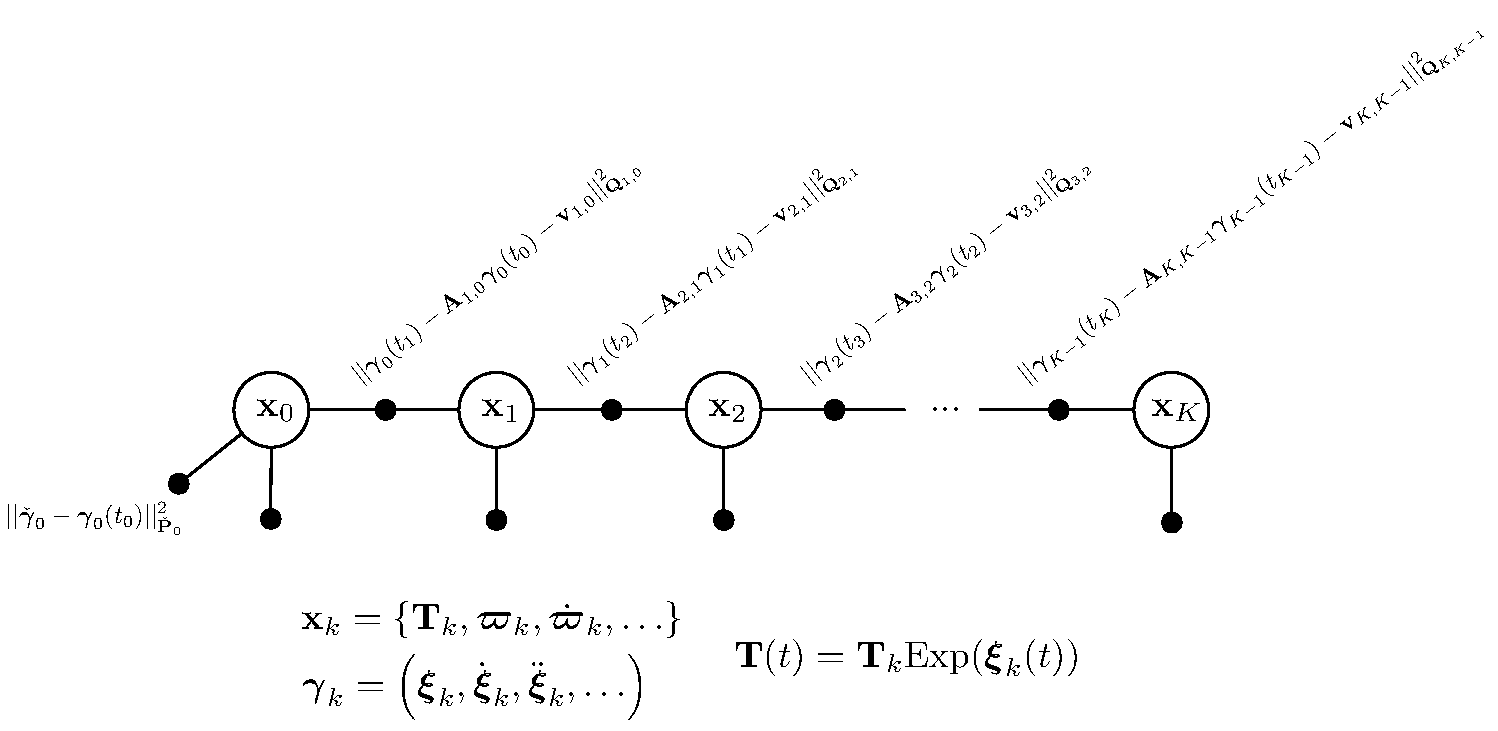
\includegraphics[width=\textwidth]{lgfg.pdf}
     \caption{General form of a motion prior defined over a Lie group trajectory.  Between each pair of measurement times, we use a linear motion model in the Lie algebra.}
     \label{fig:lgfg}
\end{figure}

To stitch several of these models together, for example one per measurement time, we can redefine $\mbs{\xi}(t)$ to be
\begin{equation}
\mbs{\xi}_k(t) = \mbox{Log} \left(\mbs{T}_k^{-1} \mbs{T}(t)\right),
\end{equation}
where $\mbs{T}_k$ is the Lie group element at the $k$th measurement time.  Then, from one measurement time to the next, we can write
\begin{multline}
p\left(\mbs{\gamma}_{k-1}(t_k) | \mbs{\gamma}_{k-1}(t_{k-1}), \mbf{v}_{k,k-1}\right) \\ = \mathcal{N}\left( \mbf{A}_{k,k-1} \mbs{\gamma}_{k-1}(t_{k-1}) + \mbf{v}_{k,k-1}, \mbf{Q}_{k,k-1}\right),
\end{multline}
recalling our linear results to compute $\mbf{A}_{k,k-1}$, $\mbf{v}_{k,k-1}$, and $\mbf{Q}_{k,k-1}$.  Our negative log-likelihood cost term is then
\begin{equation}
|| \mbs{\gamma}_{k-1}(t_k) - \mbf{A}_{k,k-1} \mbs{\gamma}_{k-1}(t_{k-1}) - \mbf{v}_{k,k-1} ||_{\mbf{Q}_{k,k-1}}^2.
\end{equation}
We can leave our motion model in this form and rely on the chain rule during optimization, but we can also work directly with the Lie group elements by substituting out the $\mbs{\gamma}_k(t)$ variables.  For example, if we want to use \ac{WNOA} as our motion model, we can substitute in the definitions of $\mbs{\xi}_k(t)$ to see that
\begin{equation}
\mbs{\gamma}_{k-1}(t) = \bbm \mbox{Log} \left(\mbs{T}_{k-1}^{-1} \mbs{T}(t)\right) \\ \mbs{J}\left(\mbox{Log} \left(\mbs{T}_{k-1}^{-1} \mbs{T}(t)\right)\right)^{-1} \mbs{\varpi}(t) \ebm,
\end{equation}
and in turn
\begin{equation}
\mbs{\gamma}_{k-1}(t_k) = \bbm \mbox{Log} \left(\mbs{T}_{k-1}^{-1} \mbs{T}_k\right) \\ \mbs{J}\left(\mbox{Log} \left(\mbs{T}_{k-1}^{-1} \mbs{T}_k\right)\right)^{-1} \mbs{\varpi}_k \ebm, \quad \mbs{\gamma}_{k-1}(t_{k-1}) = \bbm \mbf{0} \\ \mbs{\varpi}_{k-1} \ebm.
\end{equation}
Putting it all together, the negative log-likelihood cost term becomes
\begin{equation}
\left|\left| \bbm \mbox{Log} \left(\mbs{T}_{k-1}^{-1} \mbs{T}_k\right) - t_{k,k-1} \mbs{\varpi}_{k-1} \\ \mbs{J}\left(\mbox{Log} \left(\mbs{T}_{k-1}^{-1} \mbs{T}_k\right)\right)^{-1} \mbs{\varpi}_k - \mbs{\varpi}_{k-1} \ebm \right|\right|_{\mbf{Q}_{k,k-1}}^2.
\end{equation}
The top row is comparing the change in $\mbs{T}(t)$ to the generalized velocity times the time difference, while the bottom row is essentially comparing the generalized velocity at the two times.  Figure~\ref{fig:lgfg} shows the general form of a motion prior defined over a Lie group trajectory.


\section{Main Solve}

\section{Interpolation}

\section{Example}

%!TEX root =  FnTarticle.tex

\chapter{Robotics Examples in GTSAM}
\section{GTSAM Primer} 
\section{1D: Giant Glass of Milk Dataset}
\section{2D: Lost in the Woods Dataset}
\section{3D: Starry Night Dataset}

%!TEX root =  FnTarticle.tex

\chapter{Conclusion and Outlook}


%BACKMATTER SEE DOCUMENTATION
\backmatter  % references, restarts sample

\chapter{Appendices}

\printbibliography

\end{document}
